\begin{frame}[fragile]{Bad Style Coding as a Game}
  \begin{block}{The International Obfuscated C Code Contest
      (\url{www.ioccc.org})} 
    \begin{itemize}
    \item Yearly contest of intentionally obfuscated codes 
      {\small(in C; exist for other languages)}
    \end{itemize}
  \end{block}
  \begin{block}{Example: \visible<2->{Full (interactive) Maze Escape Game}
      {\normalsize (arachnid, 2004 entry)}}\vspace{-.8\baselineskip}
    \begin{columns}
      \begin{column}{.6\linewidth}
    \vbox{\begin{Verbatim}[fontsize=\tiny]
#include <ncurses.h>/*****************************************************/
            int               m[256                   ] [         256   ],a
 ,b   ;;;   ;;;   WINDOW*w;   char*l=""   "\176qxl"   "q"   "q"   "k"   "w\
xm"   "x"   "t"         "j"         "v"         "u"         "n"         ,Q[
 ]=   "Z"   "pt!ftd`"   "qdc!`eu"   "dq!$c!nnwf"/**   ***   */"t\040\t";c(
int   u ,         int         v){                     v?m   [u]         [v-
 1]   |=2,m[u][v-1] &   48?W][v-1   ] &   15]]):0:0;u?m[u   -1][v]|=1   ,m[
 u-               1][   v]&         48?               W-1   ][v         ]&
15]   ]):0:0;v<   255   ?m[   u][v+1]|=8,m[u][v+1]&   48?   W][   v+1]&15]]
):0         :0;         u <               255   ?m[   u+1         ][v   ]|=
4,m[u+1][   v]&48?W+1][v]&15]]):0:0;W][   v]&   15]   ]);}cu(char*q){   return
 *q               ?cu   (q+         1)&         1?q   [0]               ++:
q[0   ]--   :1;   }d(   int   u ,   int/**/v,   int/**/x,   int   y){   int
Y=y   -v,   X=x         -u;   int         S,s   ;Y<         0?Y   =-Y   ,s,
s=-   1:(   s=1);X<0?X=-X,S   =-1  :(S=   1);   Y<<=   1;X<<=1;   if(X>Y){
int   f=Y               -(X   >>1   );;               while(u!=         x){
f>=   0?v+=s,f-=X:0;u   +=S   ;f+=   Y;m[u][v]|=32;mvwaddch(w,v   ,u,   m[u
 ][               v]&   64?   60:         46)         ;if         (m[   u][
v]&16){c(u,v);;   ;;;   ;;;   return;}}   }else{int   f=X   -(Y>>1);;   while
 (v   !=y         ){f   >=0         ?u   +=S,               f-=         Y:0
 ;v   +=s   ;f+=X;m[u][v]|=   32;mvwaddch(w,v   ,u,m[u][v]&64?60:46);if(m[u
 ][                     v]&         16)   {c(   u,v                     );
  ;   return;;;}}}}Z(   int/**/a,   int   b){   }e(   int/**/y,int/**/  x){
int               i ;         for         (i=         a;i               <=a
+S;i++)d(y,x,i,b),d(y,x,i,b+L);for(i=b;i<=b+L;i++)d(y,x,a,i),d(y,x,a+   S,i
 );                     ;;;         ;;;         ;;;               ;;;   ;
  mvwaddch(w,x,y,64);   ;;;   ;;;   ;;;   prefresh(   w,b,a,0,0   ,L-   1,S-1
);}             main(         int               V ,   char              *C[
  ]   ){FILE*f=   fopen(V==1?"arachnid.c"/**/   :C[   1],"r");int/**/x,y,c,
                 (source code cut here)
    \end{Verbatim}
  }%$
      \end{column}
      \begin{column}{.4\linewidth}%~\medskip
        \visible<3->{
          \begin{block}{Screenshoot}\medskip
            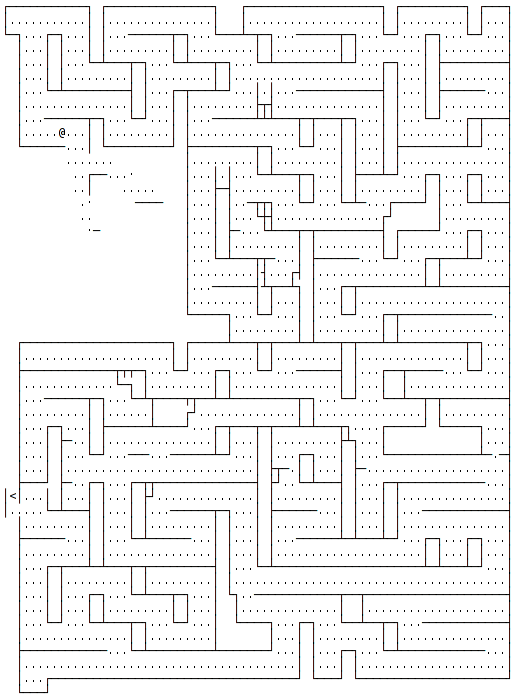
\includegraphics[width=\linewidth]{img/maze.png}          
          \end{block}
        }
      \end{column}
    \end{columns}

  \end{block}
\end{frame}
%%%%%%%%%%%%%%%%%%%%%%%%%%%%%%%%%%%%%%%%%%%%%%%%%%%%%%%%%%%%%%%%%%%%%%%
%%
%% Pas possible de faire apparaitre des Verbatim en animation
%%   => dupplication du source (irk!)
%%
\begin{frame}<handout:0>[fragile,t]{Bad Style Coding as an Art}
  \begin{block}{Another example\visible<2->{: Computing Interger Square Roots}}
    \medskip
    \begin{columns}
      \begin{column}{.3\linewidth}        
    \begin{Verbatim}[fontsize=\scriptsize]
#include <stdio.h>
int l;int main(int o,char **O,
int I){char c,*D=O[1];if(o>0){
for(l=0;D[l              ];D[l
++]-=10){D   [l++]-=120;D[l]-=
110;while   (!main(0,O,l))D[l]
+=   20;   putchar((D[l]+1032)
/20   )   ;}putchar(10);}else{
c=o+     (D[I]+82)%10-(I>l/2)*
(D[I-l+I]+72)/10-9;D[I]+=I<0?0
:!(o=main(c/10,O,I-1))*((c+999
)%10-(D[I]+92)%10);}return o;}     
    \end{Verbatim}
      \end{column}
      \begin{column}{.32\linewidth}        
        \visible<2->{\structure{It actually works}\\
        \fbox{\vbox{\scriptsize\texttt{\noindent
\$ ./cheong 1234\\
35}}}\\
{\scriptsize($35\times 35=1225$; $35\times 36=1296$)}\\
\medskip\fbox{\vbox{\scriptsize\texttt{\noindent
\$ ./cheong 112233445566\\
335012}}}\\
{\scriptsize$335012\times 335012=112233040144$
$335013\times 335013=112233710169$
}}
      \end{column}
      \begin{column}{.25\linewidth}
      \end{column}
    \end{columns}
  \end{block}

\end{frame}
\begin{frame}[fragile,t]{Bad Style Coding as an Art}
  \begin{block}{Another example: Computing Interger Square Roots}
    \medskip
    \begin{columns}
      \begin{column}{.3\linewidth}        
    \begin{Verbatim}[fontsize=\scriptsize]
#include <stdio.h>
int l;int main(int o,char **O,
int I){char c,*D=O[1];if(o>0){
for(l=0;D[l              ];D[l
++]-=10){D   [l++]-=120;D[l]-=
110;while   (!main(0,O,l))D[l]
+=   20;   putchar((D[l]+1032)
/20   )   ;}putchar(10);}else{
c=o+     (D[I]+82)%10-(I>l/2)*
(D[I-l+I]+72)/10-9;D[I]+=I<0?0
:!(o=main(c/10,O,I-1))*((c+999
)%10-(D[I]+92)%10);}return o;}     
    \end{Verbatim}
      \end{column}
      \begin{column}{.32\linewidth}        
        \structure{It actually works}\\
        \fbox{\vbox{\scriptsize\texttt{\noindent
\$ ./cheong 1234\\
35}}}\\
{\scriptsize($35\times 35=1225$; $35\times 36=1296$)}\\
\medskip\fbox{\vbox{\scriptsize\texttt{\noindent
\$ ./cheong 112233445566\\
335012}}}\\
{\scriptsize$335012\times 335012=112233040144$
$335013\times 335013=112233710169$
}
      \end{column}
      \begin{column}{.25\linewidth}
        \structure{Author claim: code self-documented$\ldots$}

        \begin{Verbatim}[fontsize=\tiny]
#include <stdio.h>
int l;int main(int o,char **O,
int I){char c,*D=O[1];if(o>0){
for(l=0;D[l              ];D[l
++]-=10){D   [l++]-=120;D[l]-=
110;while   (!main(0,O,l))D[l]
+=   20;   putchar((D[l]+1032)
/20   )   ;}putchar(10);}else{
c=o+     (D[I]+82)%10-(I>l/2)*
(D[I-l+I]+72)/10-9;D[I]+=I<0?0
:!(o=main(c/10,O,I-1))*((c+999
)%10-(D[I]+92)%10);}return o;}               
        \end{Verbatim}
      \end{column}
    \end{columns}
  \end{block}

  \visible<2->{
  \begin{boitequote}{William Strunk, Jr. (1918)}
    It is an old observation that the best writers sometimes disregard the
    rules of rhetoric.  When they do so, however, the reader will usually find
    in the sentence some compensating merit, attained at the cost of the
    violation. Unless he is certain of doing as well, he \textbf{will probably
      do best to follow the rules}.
  \end{boitequote}}
\end{frame}
